\begin{figure}[ht] 
 	\centering 
 	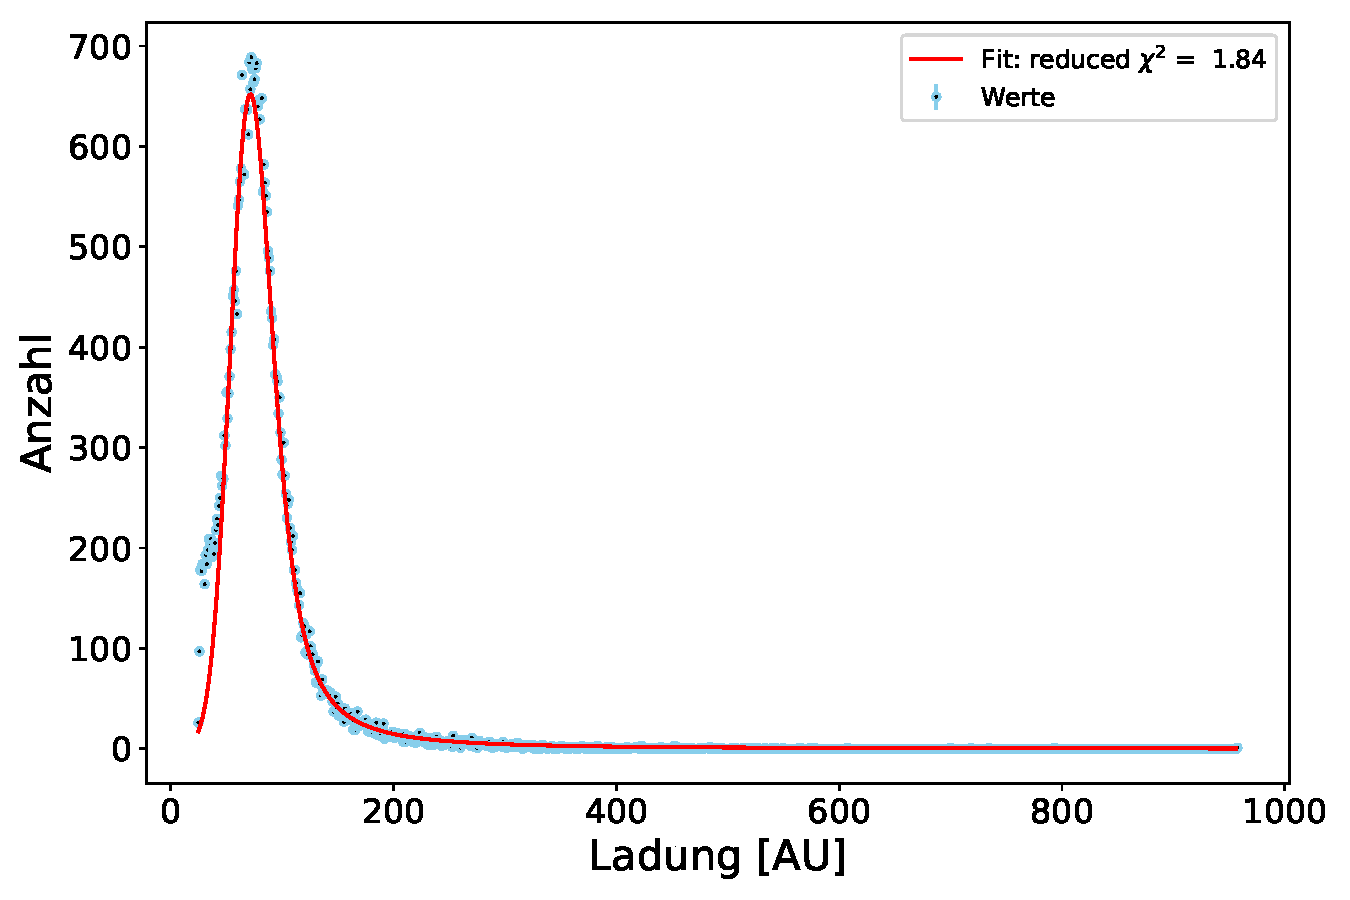
\includegraphics[width= 0.65 \textwidth]{Fits/A4_V20.h5_charge.txt_Fit.pdf} 
	\caption{A4_V20.h5_charge.txt, Fit} 
 	\label{fig:A4_V20.h5_charge.txt, Fit} 
\end{figure}
 \\ 
\begin{align} 
 	 f(x, sigma, nu, amplitude) = \frac{\sqrt{2} amplitude e^{- \frac{\left(- \nu + x\right)^{2}}{2 \sigma^{2}}}}{2 \sqrt{\pi} \sigma}
\end{align} 
\begin{table}[ht] 
\centering 
\caption{A4_V20.h5_charge.txt, Fit Parameter Tabelle} 
\label{tab:my-table}
\begin{tabular}{|l|c|}
\hline
Parameter Name	&	Wert \\ \hline
amplitude	&	 37272.570 \pm  359.228\\ \hline
center	&	 74.486 \pm  0.27\\ \hline
sigma	&	 26.080 \pm  0.248\\ \hline
fwhm	&	 61.413 \pm  0.585\\ \hline
height	&	 570.164 \pm  7.186\\ \hline
\end{tabular} 
\end{table}